\documentclass[format=sigconf]{acmart}

\usepackage{listings}
\usepackage{xcolor}

\lstset{
	basicstyle=\ttfamily\Small,
	keywordstyle=\color{blue},
	commentstyle=\color{green!50!black},
	stringstyle=\color{red},
	numbers=left,
	numberstyle=\tiny,
	numbersep=8pt,
	frame=single,
	breaklines=true,
	showstringspaces=false
}

\title{Enhancing the EEG signals visualization}

\author{André Furlan}

\affiliation{
	\institution{UNESP - Universidade Estadual Paulista Júlio de Mesquita Filho}
	\city{São José do Rio Preto}
	\state{André Furlan}
	\country{Brazil}
}
\email{ensismoebius@gmail.com}

\begin{document}
	
	\begin{abstract}
		Electroencephalogram (EEG) data has inherent complexity, including a large volume, diverse frequencies (e.g., $\alpha$, $\beta$, $\theta$, $\sigma$), and numerous emitting sources (neurons). Additionally, potential electromagnetic interferences from external sources pose challenges during EEG analysis. This work aims to propose effective visualization techniques for EEG data, drawing insights from recent research on EEG visualization. The goal is to create informative visualizations that aid in EEG research by showing detailed representations of the data without the use of misleading gradients. The visualization will include interactive features for subject and stimulus selection, providing a comprehensive understanding of EEG signals with high-contrast color schemes to enhance perceptual clarity.
	\end{abstract}
	
	\maketitle
	
	\section{Introduction}
		\par Electroencephalogram (EEG) data is widely used in neuroscience research to study brain activity. EEG records electrical signals generated by brain neurons during a task making it a valuable tool in various applications, including Brain-Computer Interfaces (BCI) and clinical diagnosis of neurological states \cite{8937083}. Analyzing EEG data, however, poses challenges due to its complexity, such as a vast number of emitting sources (neurons) and potential electromagnetic interferences from external sources like cell phones, electric motors, and magnetic fields from wires \cite{8937083}. To facilitate EEG data interpretation and visualization, it is crucial to develop effective and efficient techniques that allow researchers to gain valuable insights from the data. This paper proposes a visualization method for EEG data, combining line graphs and energy visualizations with a display of the electrode positions in the 10-20 system \cite{sistema10-20}. The proposed visualization will be interactive, allowing users to select subjects and stimuli and explore signal details. The goal is to provide researchers with an informative and comprehensive view of EEG data to support their investigations.
	
	\section{Data Acquisition}
	
		\par To demonstrate the proposed visualization technique, EEG data was acquired from an existing dataset. The chosen dataset is the "Open access database of EEG signals recorded during imagined speech" \cite{10.1117/12.2255697}. This dataset contains EEG recordings during the imagined pronunciation of vowels and commands, as well as EEG and audio recordings during the actual pronunciation. The dataset includes recordings from 15 Argentinian volunteers between the ages of 24 and 28, with an equal representation of males and females \cite{10.1117/12.2255697}.\newline
	
		\par As shown in Figure \ref{fig:sistema10-20}, the data was acquired using the 10-20 system \cite{sistema10-20} which consist of electrodes spaced by 20\% of the head size and a margin of 10\% in relation to \textit{nasion}, \textit{inion} and to the preauricular point. In this specific database only the electrodes $F3$, $F4$, $C3$, $C4$, $P3$ and $P4$ was used.
		
		\begin{figure}[h]
			\centering
			\caption{system 10-20: The electrodes are evenly separated across the scalp of the subject. The A1 electrode is the preauricular point. Source: \cite{sistema10-20}}
			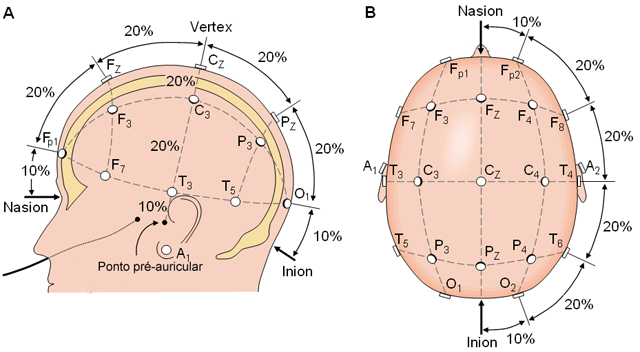
\includegraphics[width=\linewidth]{../presentation/images/sistema10-20}
			\label{fig:sistema10-20}
		\end{figure}
		
		\par Although this dataset serves as the initial data source for the proposed visualization, our future research intends to develop a custom EEG database in collaboration with local health institutions.
	
	\section{Database Structure}
		\par Each row in the dataset corresponds to a subject-stimuli-modality set, and the data is arranged as follows: EEG signals from different electrodes, modalities (imagined or pronounced), and stimulus codes representing different categories of stimuli (e.g., letters and commands). The modalities distinguish between imagined and pronounced speech, while the stimulus codes identify specific categories of stimuli. Figure \ref{fig:visu04} shows a sample of the initial rows in the database, and Figure \ref{fig:visu05} displays the last rows.\newline
		
		\par Being F3, F4, C3, C4, P3 and P4 the name of the electrodes in the 10-20 system, each line consist in a series of numbers organized as follows:
		
		\begin{itemize}
			\item F3 - 0:4095
			\item F4 - 4096:8191
			\item C3 - 8192:12287
			\item C4 - 12288:16383
			\item P3 - 16384:20479
			\item P4 - 20480:24575
			\item modality - 24576:24576
			\item estimuli - 24577:24577
			\item artifact - 24578:24578
		\end{itemize}
	
		\par Modality can be 1 for imagined speech or 2 for pronounced speech. Stimuli assumes 1: A, 2: E, 3: I, 4:O and 5:U and 6:\textit{Arriba}, 7: \textit{Abajo}, 8: \textit{Adelante}, 9: \textit{Atrás}, 10: \textit{Derecha}, 11: \textit{Izquierda} finally artifact assumes 1 for no eye blinking and 2 otherwise.
		
		\begin{figure}[h]
			\centering
			\caption{Sample of initial rows in the EEG database}
			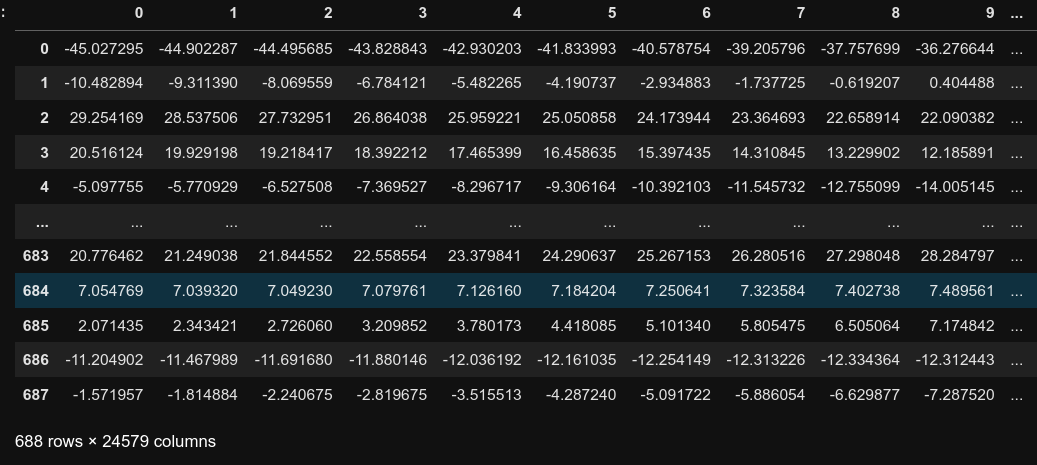
\includegraphics[width=\linewidth]{../presentation/images/visu04}
			\label{fig:visu04}
		\end{figure}
		
		\begin{figure}[h]
			\centering
			\caption{Sample of last rows in the EEG database}
			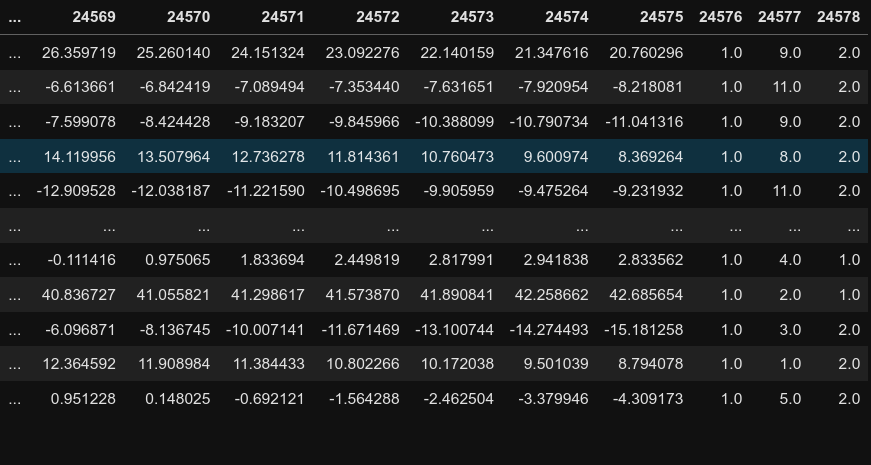
\includegraphics[width=.9\linewidth]{../presentation/images/visu05}
			\label{fig:visu05}
		\end{figure}
	
	\section{Preprocessing}
		\par To facilitate data manipulation and visualization, pre-processing techniques are applied to the EEG data. The data is grouped and organized to ensure better interactions and efficient representation. Figure \ref{fig:visu06} demonstrates the pre-processed and grouped data, ready for visualization.
	
		\begin{figure}[h]
			\centering
			\caption{Pre-processed and Grouped EEG Data: Note the columns named after its respective source (i.e., the electrodes) and the last three ones "modalidade," "Estímulo," and "Artefatos," which are, respectively, the modality, stimuli and artifacts.}
			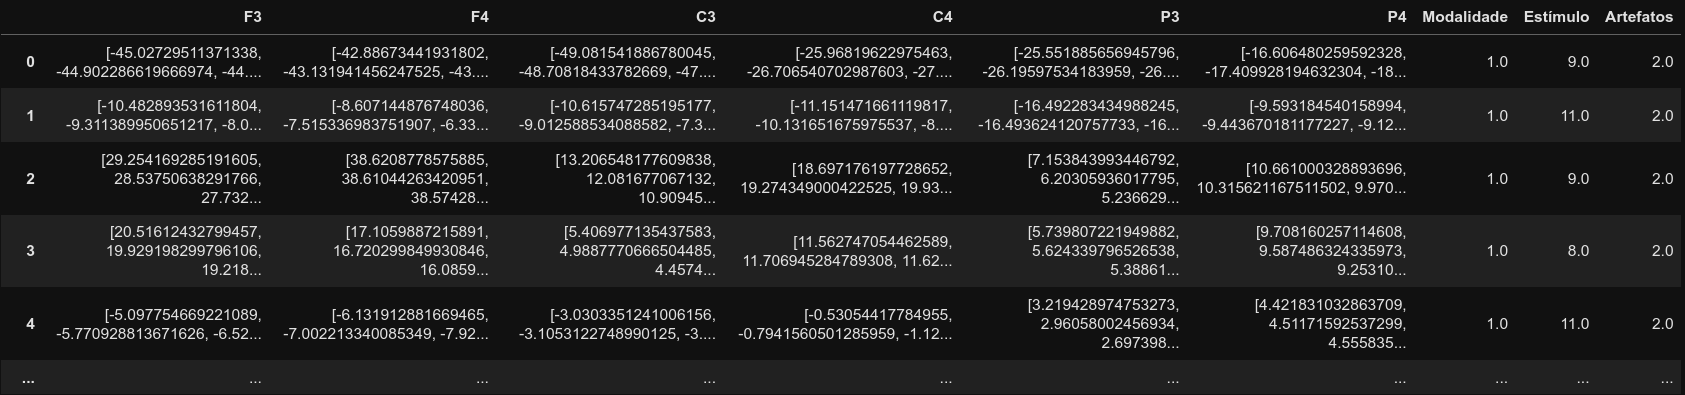
\includegraphics[width=\linewidth]{../presentation/images/visu06}
			\label{fig:visu06}
		\end{figure}
	
	\section{Case Studies}
		\par The proposed visualization method drew inspiration from case studies that utilized real EEG data. These case studies focused on various subjects and stimuli, showcasing their effectiveness and utility. Accordingly, certain features will be incorporated, while others will be discarded.
	
		\subsection{Visualization: EPviz \cite{currey2023epviz}}
			\par EPviz uses line graphs to visualize EEG data \cite{currey2023epviz} and provide a general overview of the data. The visualization by lines is efficient because it shows the high and low frequency components. In the example shown in Figure \ref{fig:epviz00}, the EPViz program visualizes the signals captured by all the electrodes, providing a good overview. However, it lacks the detailed view that would allow a more accurate analysis of the displayed curves.			
		
			\begin{figure}[h]
				\centering
				\caption{EPviz - Line graph visualization}
				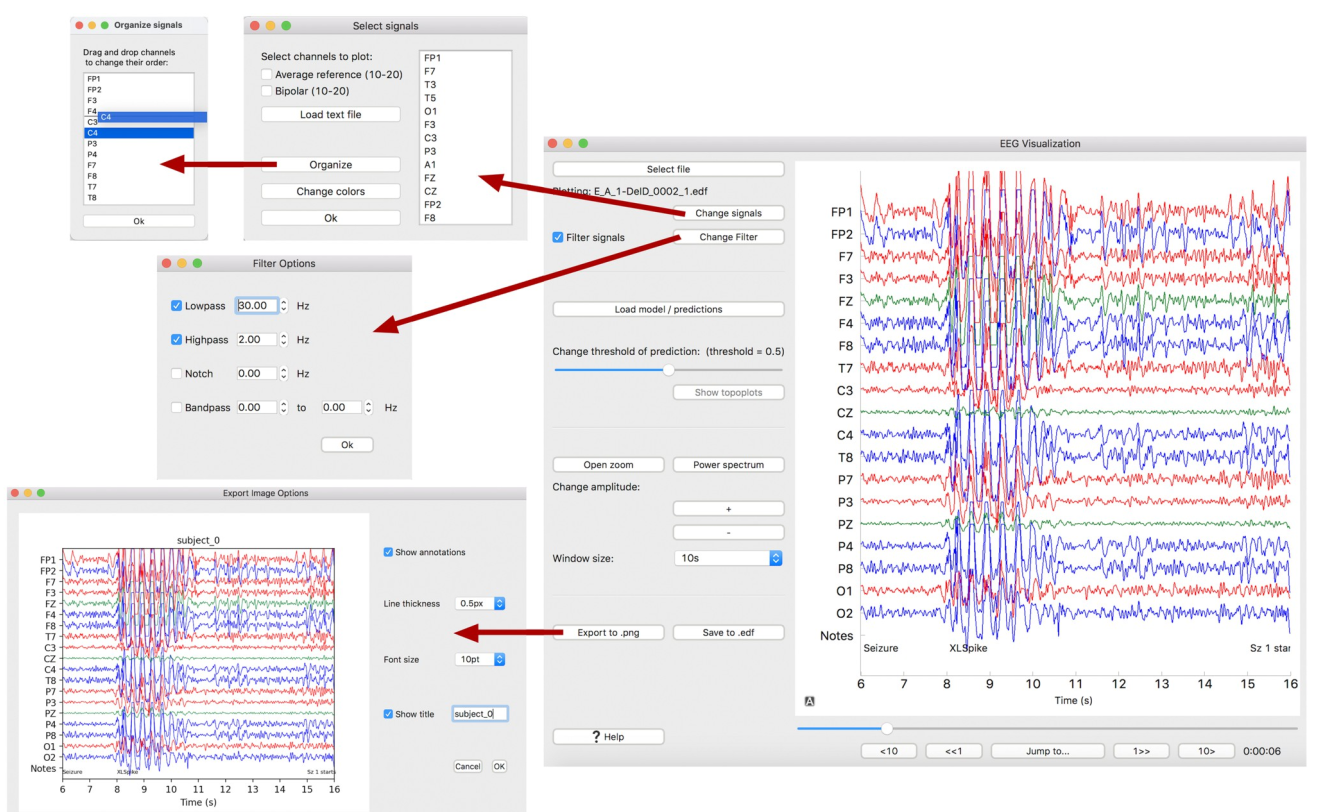
\includegraphics[width=\linewidth]{../presentation/images/epviz00}
				\label{fig:epviz00}
			\end{figure}
	
		\subsection{Visualization: Topological \cite{9098189}}
			\par Another relevant methodology uses topological color maps to indicate signal energy at each electrode. This visualization approach shown in Figure \ref{fig:visu01} provides an informative representation of regions with intense brain activity during the corresponding time period. However, the view makes a interpolation of measured values leading to potential misinterpretations of signal intensities according to gradients.
			
			\begin{figure}[h]
				\centering
				\caption{Topological visualization}
				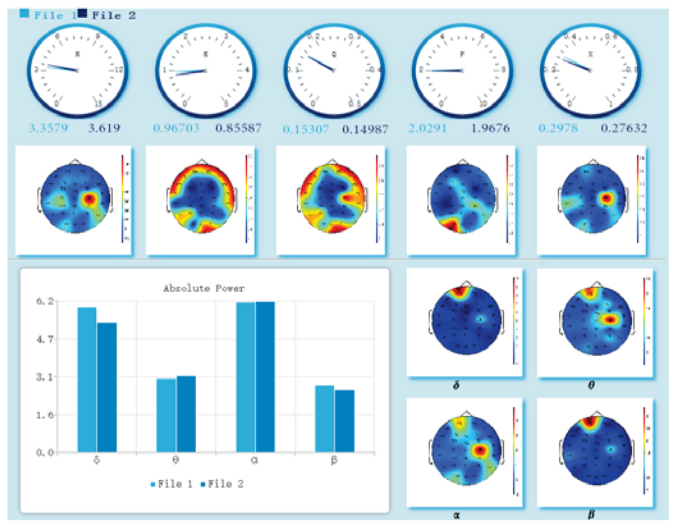
\includegraphics[width=\linewidth]{../presentation/images/visu01}
				\label{fig:visu01}
			\end{figure}
	
		\subsection{Visualization: Topological over time \cite{8937083}}
			\par The methodology shown in Figure \ref{fig:visu02} simplifies the visualization to display brain activity at four different moments. However, similar to the previous visualization, the gradient issue persists, potentially leading to incorrect interpretations.
			
			\begin{figure}[h]
				\centering
				\caption{Topological visualization over time}
				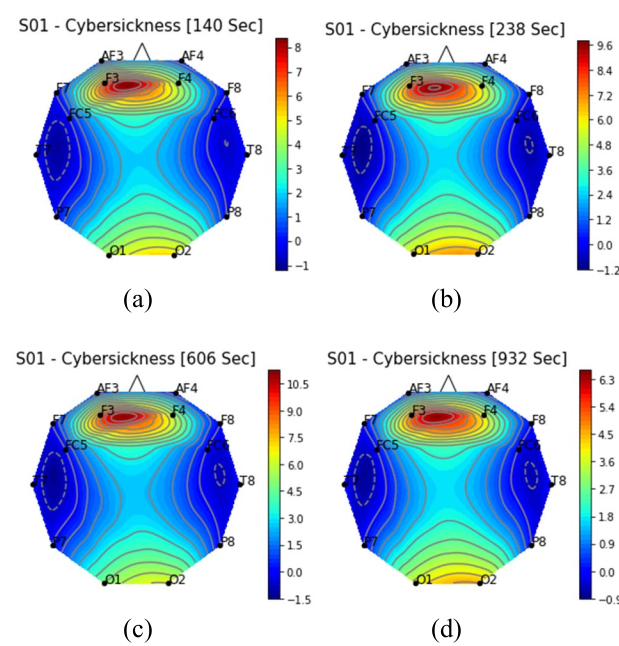
\includegraphics[width=\linewidth]{../presentation/images/visu02}
				\label{fig:visu02}
			\end{figure}
	
	\section{Proposal}
		\par The proposed visualization method includes line graphs and energy visualizations combined with a non-gradient representation of electrode positions in the 10-20 system. The interactive features allow users to select subjects and stimuli, explore specific signal details, view the signal's origin, and scale up or down the displayed curves. Additionally, the visualization will include bars showing the total energy of the displayed signal interval. The use of high-contrast colors will aid in perceptual differentiation. Figures \ref{fig:g3714} and \ref{fig:g3762} illustrate the general and specific views proposed.
	
		\begin{figure}[h]
			\centering
			\caption{Specific view of the proposed visualization}
			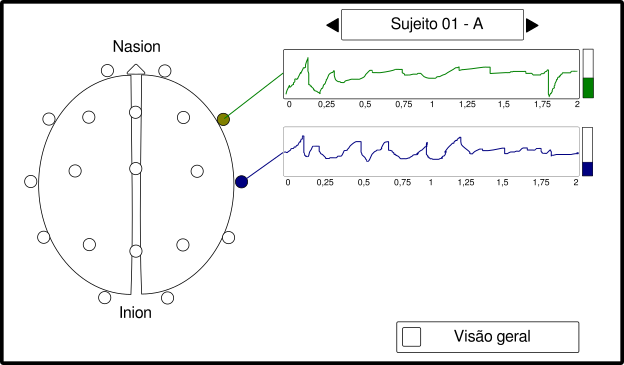
\includegraphics[width=\linewidth]{../presentation/images/g3714}
			\label{fig:g3714}
		\end{figure}
		
		\begin{figure}[h]
			\centering
			\caption{General view of the proposed visualization}
			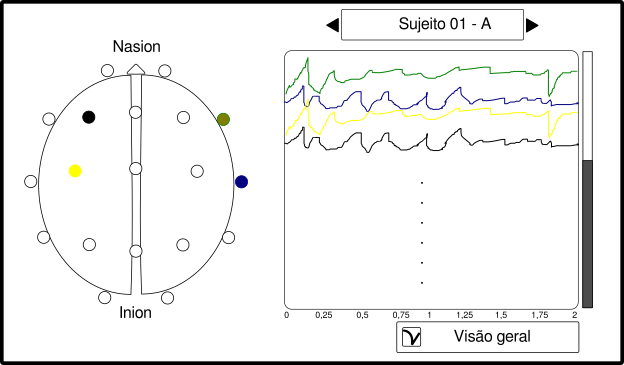
\includegraphics[width=\linewidth]{../presentation/images/g3762}
			\label{fig:g3762}
		\end{figure}
	
		\par Both the \textbf{subject and stimulus selection} and the checkbox are integral components of the \textbf{visualization cycle} \cite{munzner2014visualization}. When modifying the type of vision, stimuli and/or the analyzed subject, the view must promptly respond by updating the displayed data.\newline
		
		\par The use of \textbf{high contrast} colors aids in easily locating the origin of the data \cite{spence2014information}, preventing the common problem of differentiating data when very similar colors are employed.\newline
		
		\par The \textbf{magnification} feature enables a detailed view of each signal \cite{tufte1983visual}, facilitating the visualization of information linked to low and high-frequency signals. This provides the identification of \textbf{objects according to their "silhouette"} \cite{tufte2006beautiful}.\newline
		
		\par It's worth noting that the attributes utilized in the proposal have a \textbf{sequential} \cite{kirk2012data} order for the amplitude and frequency of the signals over time (line graphs), while simultaneously being \textbf{categorical} \cite{kirk2012data} because the frequency analysis can reveal valuable insights about the subject being analyzed.\newline
		
		\par The energy attribute (vertical bar on the side of the line graph) is \textbf{quantitative}.\newline
		
		\par Regarding \textbf{categorical} attributes, the region to the left of the graphs also deserves attention. This section indicates which brain regions are emitting specific signals, allowing, for example, the inference of the most active brain regions during thought execution and/or action.\newline
		
		
		\par In terms of \textbf{semiotic categories} \cite{santaella2017semiotica} it is possible to highlight:
		\begin{itemize}
			\item firstness: Colors that stand out and immediately call the user's attention.
			\item secondness: The action/reaction applied to controls and images.
			\item thirdness: The consequent interpretation of the image presented as well as the reasoning necessary for understanding what is shown.
		\end{itemize}
		
	\section{Implementation}
		\par The visualization was implemented using the Python3 \cite{Python3} programming language due to its extensive set of data visualization and manipulation libraries. It is important to note that the final result differs slightly from the proposal, however, this does not compromise the quality of the final product, as can be seen in Figure \ref{fig:screenshot01} and \ref{fig:screenshot02}.
		
		\begin{figure}[h]
			\centering
			\caption{The application screenshot in specific mode: All signals are represented separately.}
			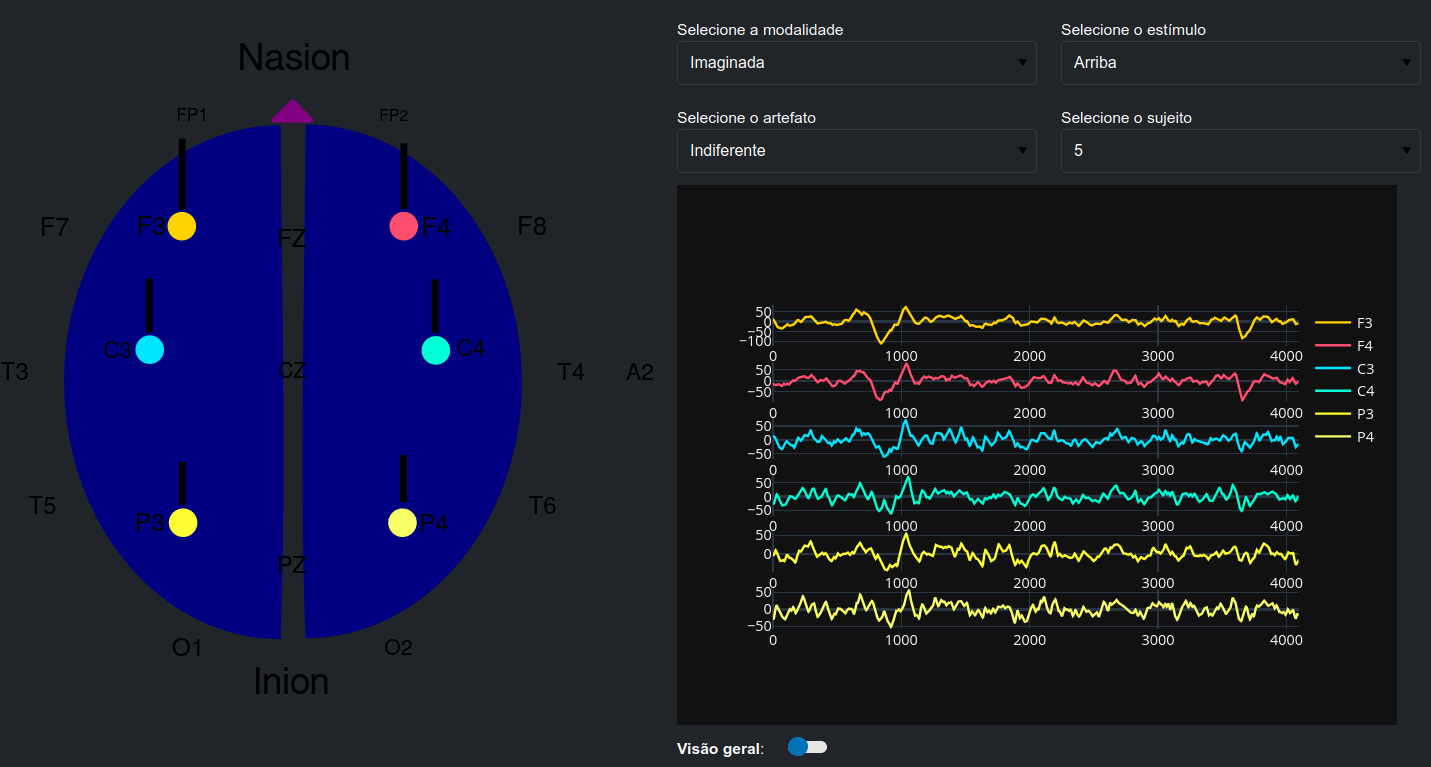
\includegraphics[width=\linewidth]{images/screenshot01}
			\label{fig:screenshot01}
		\end{figure}
		
		\begin{figure}[h]
			\centering
			\caption{The application screenshot in general mode: All signals are represented in a single plot.}
			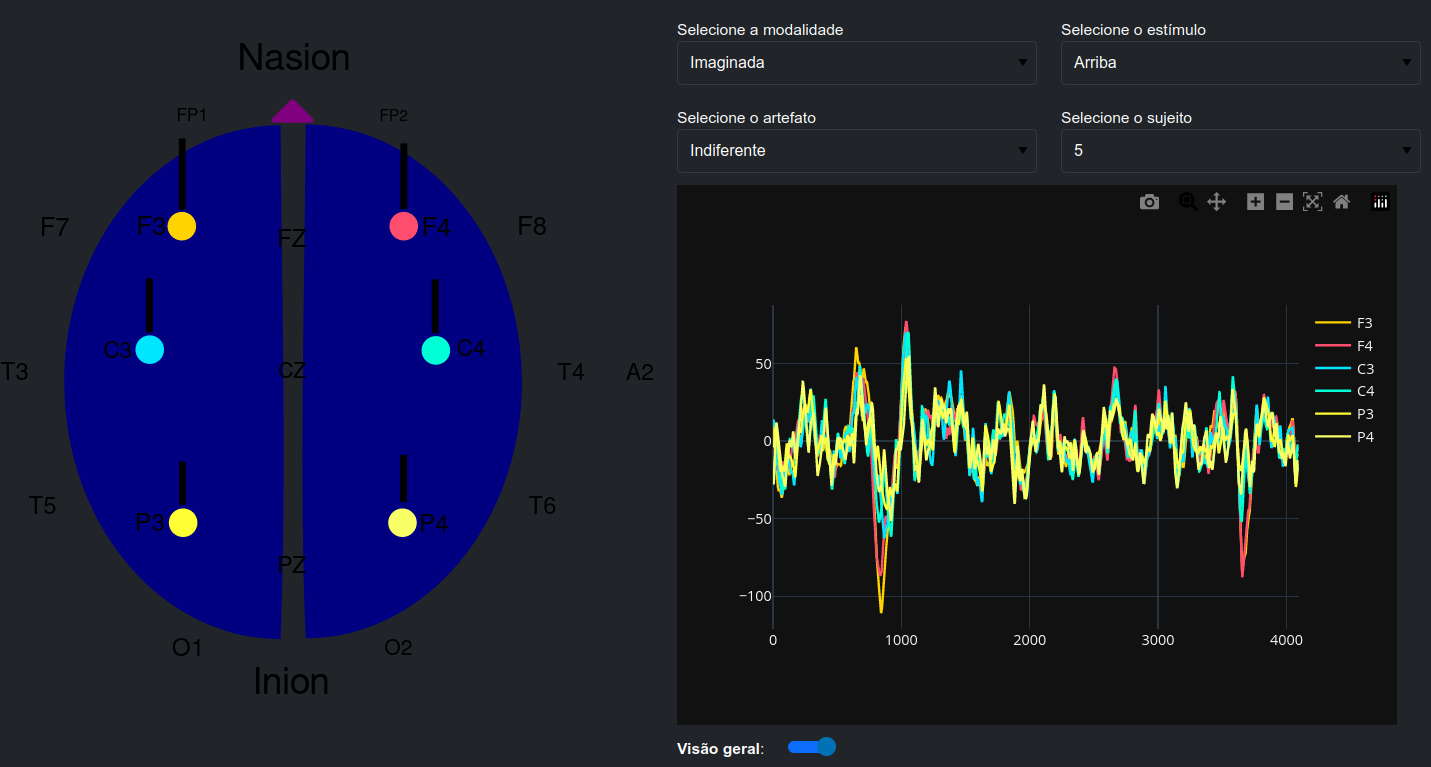
\includegraphics[width=\linewidth]{images/screenshot02}
			\label{fig:screenshot02}
		\end{figure}
	
		\subsection{User interface discussion}
			\par Focusing on the left side of the visualization: Like is shown in Figure \ref{fig:screenshotleft}, the electrodes that are being used are represented by circles with vivid and contrasting colors which matches with its respectively plot on the right side, while the unused electrodes are represented only by their names. At the top of each circle, there is a bar representing the corresponding signal's energy captured by that electrode. It is noteworthy that each signal may have different energy levels.
		
			\begin{figure}[h]
				\centering
				\caption{The electrodes and its captured energy are represented by the colored circles and their top bars respectively.}
				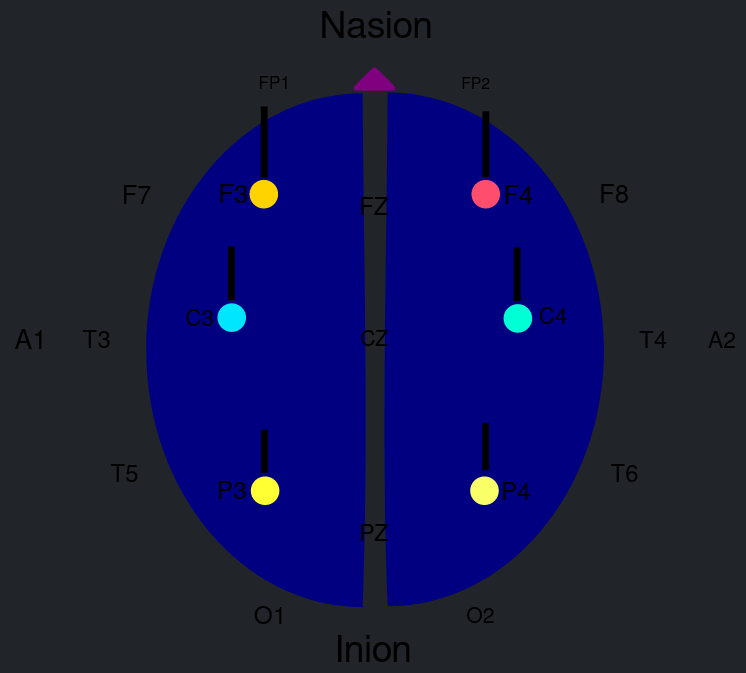
\includegraphics[width=\linewidth]{images/screenshotLeft}
				\label{fig:screenshotleft}
			\end{figure}
		
			\par The top section shown in Figure \ref{fig:screenshottop} is where the data filters reside: The first one "Selecione a modalidade" is a selector of the modality of the speech: Imagined or pronounced. Just setting this value alone does not affect the visualization because it needs the type of stimuli too. At the "Selecione o estímulo" selector is possible to set the type of stimuli which the visualization are needed. Considering that the previous selector is already set, this will trigger the change on the left and right parts of the screen showing the data visualization for the first subject. The subject can be changed using the "Selecione o sujeito" selector. Finally, the "Selecione o artefato" selector filters if data with artifacts are shown or not shown.
			
			\begin{figure}[h]
				\centering
				\caption{The four selectors of the visualization: "Selecione a modalidade", "Selecione o estímulo", "Selecione o artefato" and "Selecione o sujeito"}
				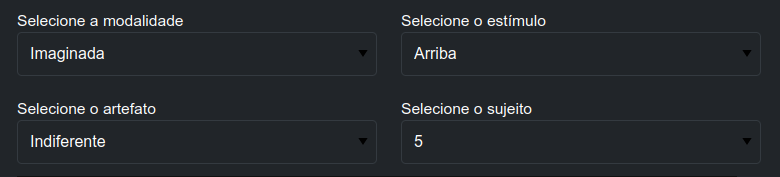
\includegraphics[width=\linewidth]{images/screenshotTop}
				\label{fig:screenshottop}
			\end{figure}
		
			
		
			\par The right section (Figure \ref{fig:screenshotright}) displays the plots of the signals captured by the electrodes. Each plot has a color matching to its respective electrode, and to avoid misinterpretations, there are labels on the right. This section changes when new filters are set and when the switch "Visão geral" depicted in Figure \ref{fig:screenshotbotton} is changed. Here, it is possible to zoom in on data, hide plots by clicking on labels, and even save the results to a file.
			
			\begin{figure}[h]
				\centering
				\caption{The right section of the visualization: The signals may be shown separately or in a single plot.}
				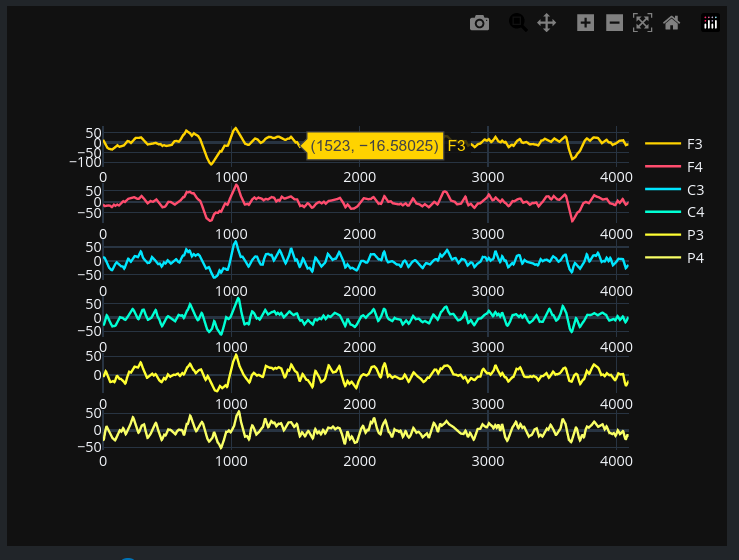
\includegraphics[width=\linewidth]{images/screenshotRight}
				\label{fig:screenshotright}
			\end{figure}
			
			
			\begin{figure}[h]
				\centering
				\caption{This button switches between "General" and "Specific" modes.}
				
\includegraphics{images/screenshotBotton}
				\label{fig:screenshotbotton}
			\end{figure}
		\subsection{Source code}
		
			\par This section provides an overview of the most important code excerpts. The full code is available in the repository listed at the end of this document. This visualization utilizes the following Python libraries: Panel, Plotly, SciPy, Pandas, BeautifulSoup, and NumPy. It comprises two main classes: \texttt{Dashdata} and \texttt{Dashboard}.\newline
			
			\par The \texttt{Dashdata} class is responsible for loading and processing EEG data. The main tasks of this class are as follows:
			
			\begin{itemize}
				
				\item{\textbf{loading EEG Data}}: The \texttt{Dashdata} class loads EEG data from a MATLAB file using the \texttt{scipy.io.loadmat} function. The EEG data is stored in a MATLAB struct format, and the class uses \texttt{squeeze\_me} and \texttt{mat\_dtype} options to convert the data into a more usable format.
	
				\lstinputlisting[language=Python, caption={Loading a Matlab file}]{code/loadEEGData.py}
			
				\item{\textbf{data preprocessing}}: After loading the data, the class creates a Pandas DataFrame called \texttt{dataframe} to store the EEG data. The EEG signals for specific electrodes are combined into arrays, and the DataFrame is updated accordingly. This step simplifies data handling and allows easier access to EEG signal data for visualization. This is done using the \textit{\_joinIntoArray} function.
				
				\lstinputlisting[language=Python, caption={This function groups the columns}]{code/dataProcessingFunc.py}
				
				\lstinputlisting[language=Python, caption={Grouping the columns}]{code/dataProcessing.py}
				
				\item{\textbf{setting up Properties}}: The class sets up properties to store essential information, such as the relationship between EEG electrodes and their corresponding colors. This mapping is useful for visualizing EEG signals with different colors representing different electrodes.
				
				\lstinputlisting[language=Python, caption={Color and sensor data}]{code/sensorData.py}
				
				\item{\textbf{mapping Modalities, Stimuli, and Artifacts}}: The \texttt{Dashdata} class provides dictionaries to map descriptive names of modalities, stimuli, and artifacts to their respective numeric codes. This mapping facilitates user interaction, as select widgets can be populated with descriptive options.
				
				\lstinputlisting[language=Python, caption={Dictionaries for widgets}]{code/widgetsDict.py}
				
				\item{\textbf{loading brain Visualization}}: The class loads an SVG image of the brain, which serves the purpose of visualizing the locations of EEG electrodes on the brain. Incorporating this SVG image into the dashboard enhances the user experience and offers context to the EEG data. An additional advantage of this approach is that, due to the handcrafted nature of this resource, it can be readily replaced by another SVG image to meet new requirements and demands!
				
				\lstinputlisting[language=Python, caption={Loading SVG image}]{code/loadSVG.py}
			\end{itemize}
			
			\par The \texttt{Dashboard} class is designed to create an interactive EEG Data Visualization Dashboard using Panel and Plotly libraries. It utilizes the \texttt{Dashdata} class to access preprocessed EEG and visual elements data.
			
			\begin{itemize}
				\item As aforementioned the SVG image is used to represent the brain. But this representation means nothing if it cannot be modified to reflect the visualization parameters. To do this two functions are used to update this image.
				
				\lstinputlisting[language=Python, caption={Functions that updates the SVG image}]{code/SVGFunc.py}
				
				
				\item{\textbf{widgets and UI Layout}} The dashboard creates various widgets for user interaction, such as selects for modalities, stimuli, artifacts, and subjects. Additionally, a switch widget is used to toggle between general and detailed views of the EEG data. The dashboard's layout is arranged using rows and columns to organize the visual elements effectively.
				
				\item{\textbf{event handling}} This class defines callback methods to handle user interactions with the widgets. These methods update the visualization based on the user's selections for modalities, stimuli, artifacts, subjects, and the general view toggle. The EEG data is filtered and plotted accordingly to provide an interactive and dynamic visualization experience.
				
				\item{\textbf{data visualization}} The dashboard uses Plotly to visualize the EEG data. It creates line plots representing EEG signals for different electrodes. Depending on the user's selection, the dashboard can display single-panel or multiple-panel plots. The latter provides a more detailed view of the EEG signals.
			\end{itemize}
	
	\section{Conclusion and future work}
		\par The non-gradient method of displaying data in conjunction with the capacity of data isolation offers more clarity and reduce misinterpretation of the data. But, despite the current state of this visualization being well-rounded, some features may be implemented: the capacity to dynamically load data in other formats, the decomposition of data into its sub-frequencies ($\alpha$, $\beta$, $\theta$, $\sigma$), and a real-time display of EEG. As research progresses, the proposed visualization will be further developed to incorporate these features. 

	\section{Code Repository}
		\par To access the source code, please visit:\newline \href{https://github.com/ensismoebius/VisualizacaoDeInformacao}{\textbf{https://github.com/ensismoebius/VisualizacaoDeInformacao}}
	
	\begin{acks}
		The author would like to thank the Universidade Estadual Paulista Júlio de Mesquita Filho for its support and resources during this research.
	\end{acks}
	
	\bibliographystyle{ACM-Reference-Format}
	\bibliography{../presentation/bibliography.bib}
	
\end{document}
